\tikzset{every picture/.style={line width=0.75pt}} %set default line width to 0.75pt        

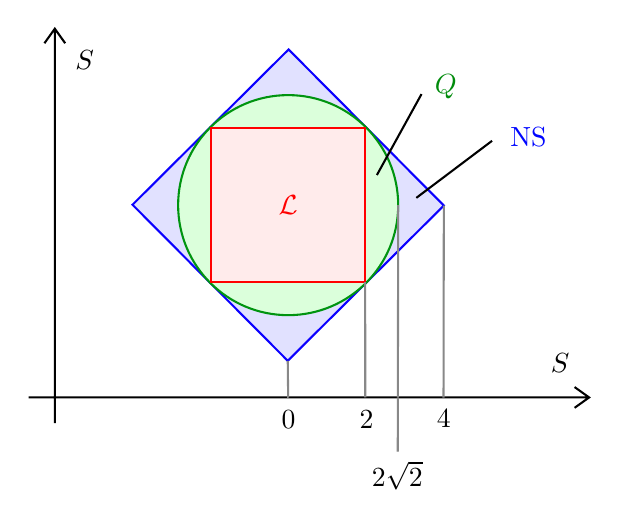
\begin{tikzpicture}[x=0.75pt,y=0.75pt,yscale=-1,xscale=1]
%uncomment if require: \path (0,300); %set diagram left start at 0, and has height of 300

%Shape: Rectangle [id:dp30928970522637145] 
\draw  [color={rgb, 255:red, 11; green, 0; blue, 255 }  ,draw opacity=1 ][fill={rgb, 255:red, 225; green, 225; blue, 255 }  ,fill opacity=1 ] (240,114.8) -- (315.2,40) -- (390,115.2) -- (314.8,190) -- cycle ;
%Shape: Ellipse [id:dp9930572540891616] 
\draw  [color={rgb, 255:red, 0; green, 148; blue, 16 }  ,draw opacity=1 ][fill={rgb, 255:red, 219; green, 255; blue, 219 }  ,fill opacity=1 ] (261.99,115) .. controls (261.99,85.72) and (285.72,61.99) .. (315,61.99) .. controls (344.28,61.99) and (368.01,85.72) .. (368.01,115) .. controls (368.01,144.28) and (344.28,168.01) .. (315,168.01) .. controls (285.72,168.01) and (261.99,144.28) .. (261.99,115) -- cycle ;
%Shape: Axis 2D [id:dp5751847689571885] 
\draw  (190,207.65) -- (460,207.65)(202.57,30) -- (202.57,220) (453,202.65) -- (460,207.65) -- (453,212.65) (197.57,37) -- (202.57,30) -- (207.57,37)  ;
%Shape: Rectangle [id:dp8277993508737616] 
\draw  [color={rgb, 255:red, 255; green, 0; blue, 0 }  ,draw opacity=1 ][fill={rgb, 255:red, 255; green, 235; blue, 235 }  ,fill opacity=1 ] (277.89,77.89) -- (352.11,77.89) -- (352.11,152.11) -- (277.89,152.11) -- cycle ;
%Straight Lines [id:da3288239217718776] 
\draw [color={rgb, 255:red, 136; green, 136; blue, 136 }  ,draw opacity=1 ][fill={rgb, 255:red, 0; green, 0; blue, 0 }  ,fill opacity=1 ]   (352.11,152.11) -- (352.14,207.57) ;


%Straight Lines [id:da5700506077210445] 
\draw [color={rgb, 255:red, 136; green, 136; blue, 136 }  ,draw opacity=1 ][fill={rgb, 255:red, 0; green, 0; blue, 0 }  ,fill opacity=1 ]   (368.01,115) -- (367.86,207.57) ;


%Straight Lines [id:da9368725092254024] 
\draw [color={rgb, 255:red, 136; green, 136; blue, 136 }  ,draw opacity=1 ][fill={rgb, 255:red, 0; green, 0; blue, 0 }  ,fill opacity=1 ]   (390,115.2) -- (389.85,207.77) ;


%Straight Lines [id:da9435052139977784] 
\draw [color={rgb, 255:red, 136; green, 136; blue, 136 }  ,draw opacity=1 ][fill={rgb, 255:red, 0; green, 0; blue, 0 }  ,fill opacity=1 ]   (367.86,207.57) -- (367.8,233.8) ;


%Straight Lines [id:da06475354051924254] 
\draw    (357.75,100.5) -- (379.25,61.5) ;


%Straight Lines [id:da9429638260774549] 
\draw    (376.75,111.5) -- (413.25,84) ;


%Straight Lines [id:da0310564865217966] 
\draw [color={rgb, 255:red, 136; green, 136; blue, 136 }  ,draw opacity=1 ][fill={rgb, 255:red, 0; green, 0; blue, 0 }  ,fill opacity=1 ]   (314.8,190) -- (315,207.8) ;



% Text Node
\draw (352.8,218.2) node   {$2$};
% Text Node
\draw (367.6,245.4) node   {$2\sqrt{2}$};
% Text Node
\draw (390,217.8) node   {$4$};
% Text Node
\draw (446,191) node   {$S$};
% Text Node
\draw (217,45) node   {$S$};
% Text Node
\draw (315,115) node [color={rgb, 255:red, 255; green, 0; blue, 0 }  ,opacity=1 ]  {$\mathcal{L}$};
% Text Node
\draw (390.9,58.14) node [color={rgb, 255:red, 1; green, 139; blue, 12 }  ,opacity=1 ]  {$Q$};
% Text Node
\draw (430.72,82.23) node [color={rgb, 255:red, 0; green, 6; blue, 255 }  ,opacity=1 ]  {$\mathrm{NS}$};
% Text Node
\draw (315.2,218.2) node   {$0$};


\end{tikzpicture}